\documentclass[12pt,a4paper,oneside]{article}
\usepackage[colorlinks=true]{hyperref}
\usepackage[utf8]{inputenc}
\usepackage[czech]{babel}
\usepackage{graphicx}
\usepackage{pdfpages}
\textwidth 16cm \textheight 25cm
\topmargin -1.3cm 
\oddsidemargin 0cm
\pagestyle{empty}
\begin{document}
\title{Generátor hodin CLKGEN01B}
\author{Jakub Kákona, kaklik@mlab.cz}
\maketitle

\thispagestyle{empty}
\begin{abstract}
Účelem tohoto modulu je poskytnout uživateli dostatečně kvalitní laditelný zdroj frekvenčně stabilního signálu s nízkým šumem vhodného pro konstrukce se špičkovými ADC a obecně v konstrukcích SDR.
\end{abstract}

\begin{figure} [htbp]
\begin{center}
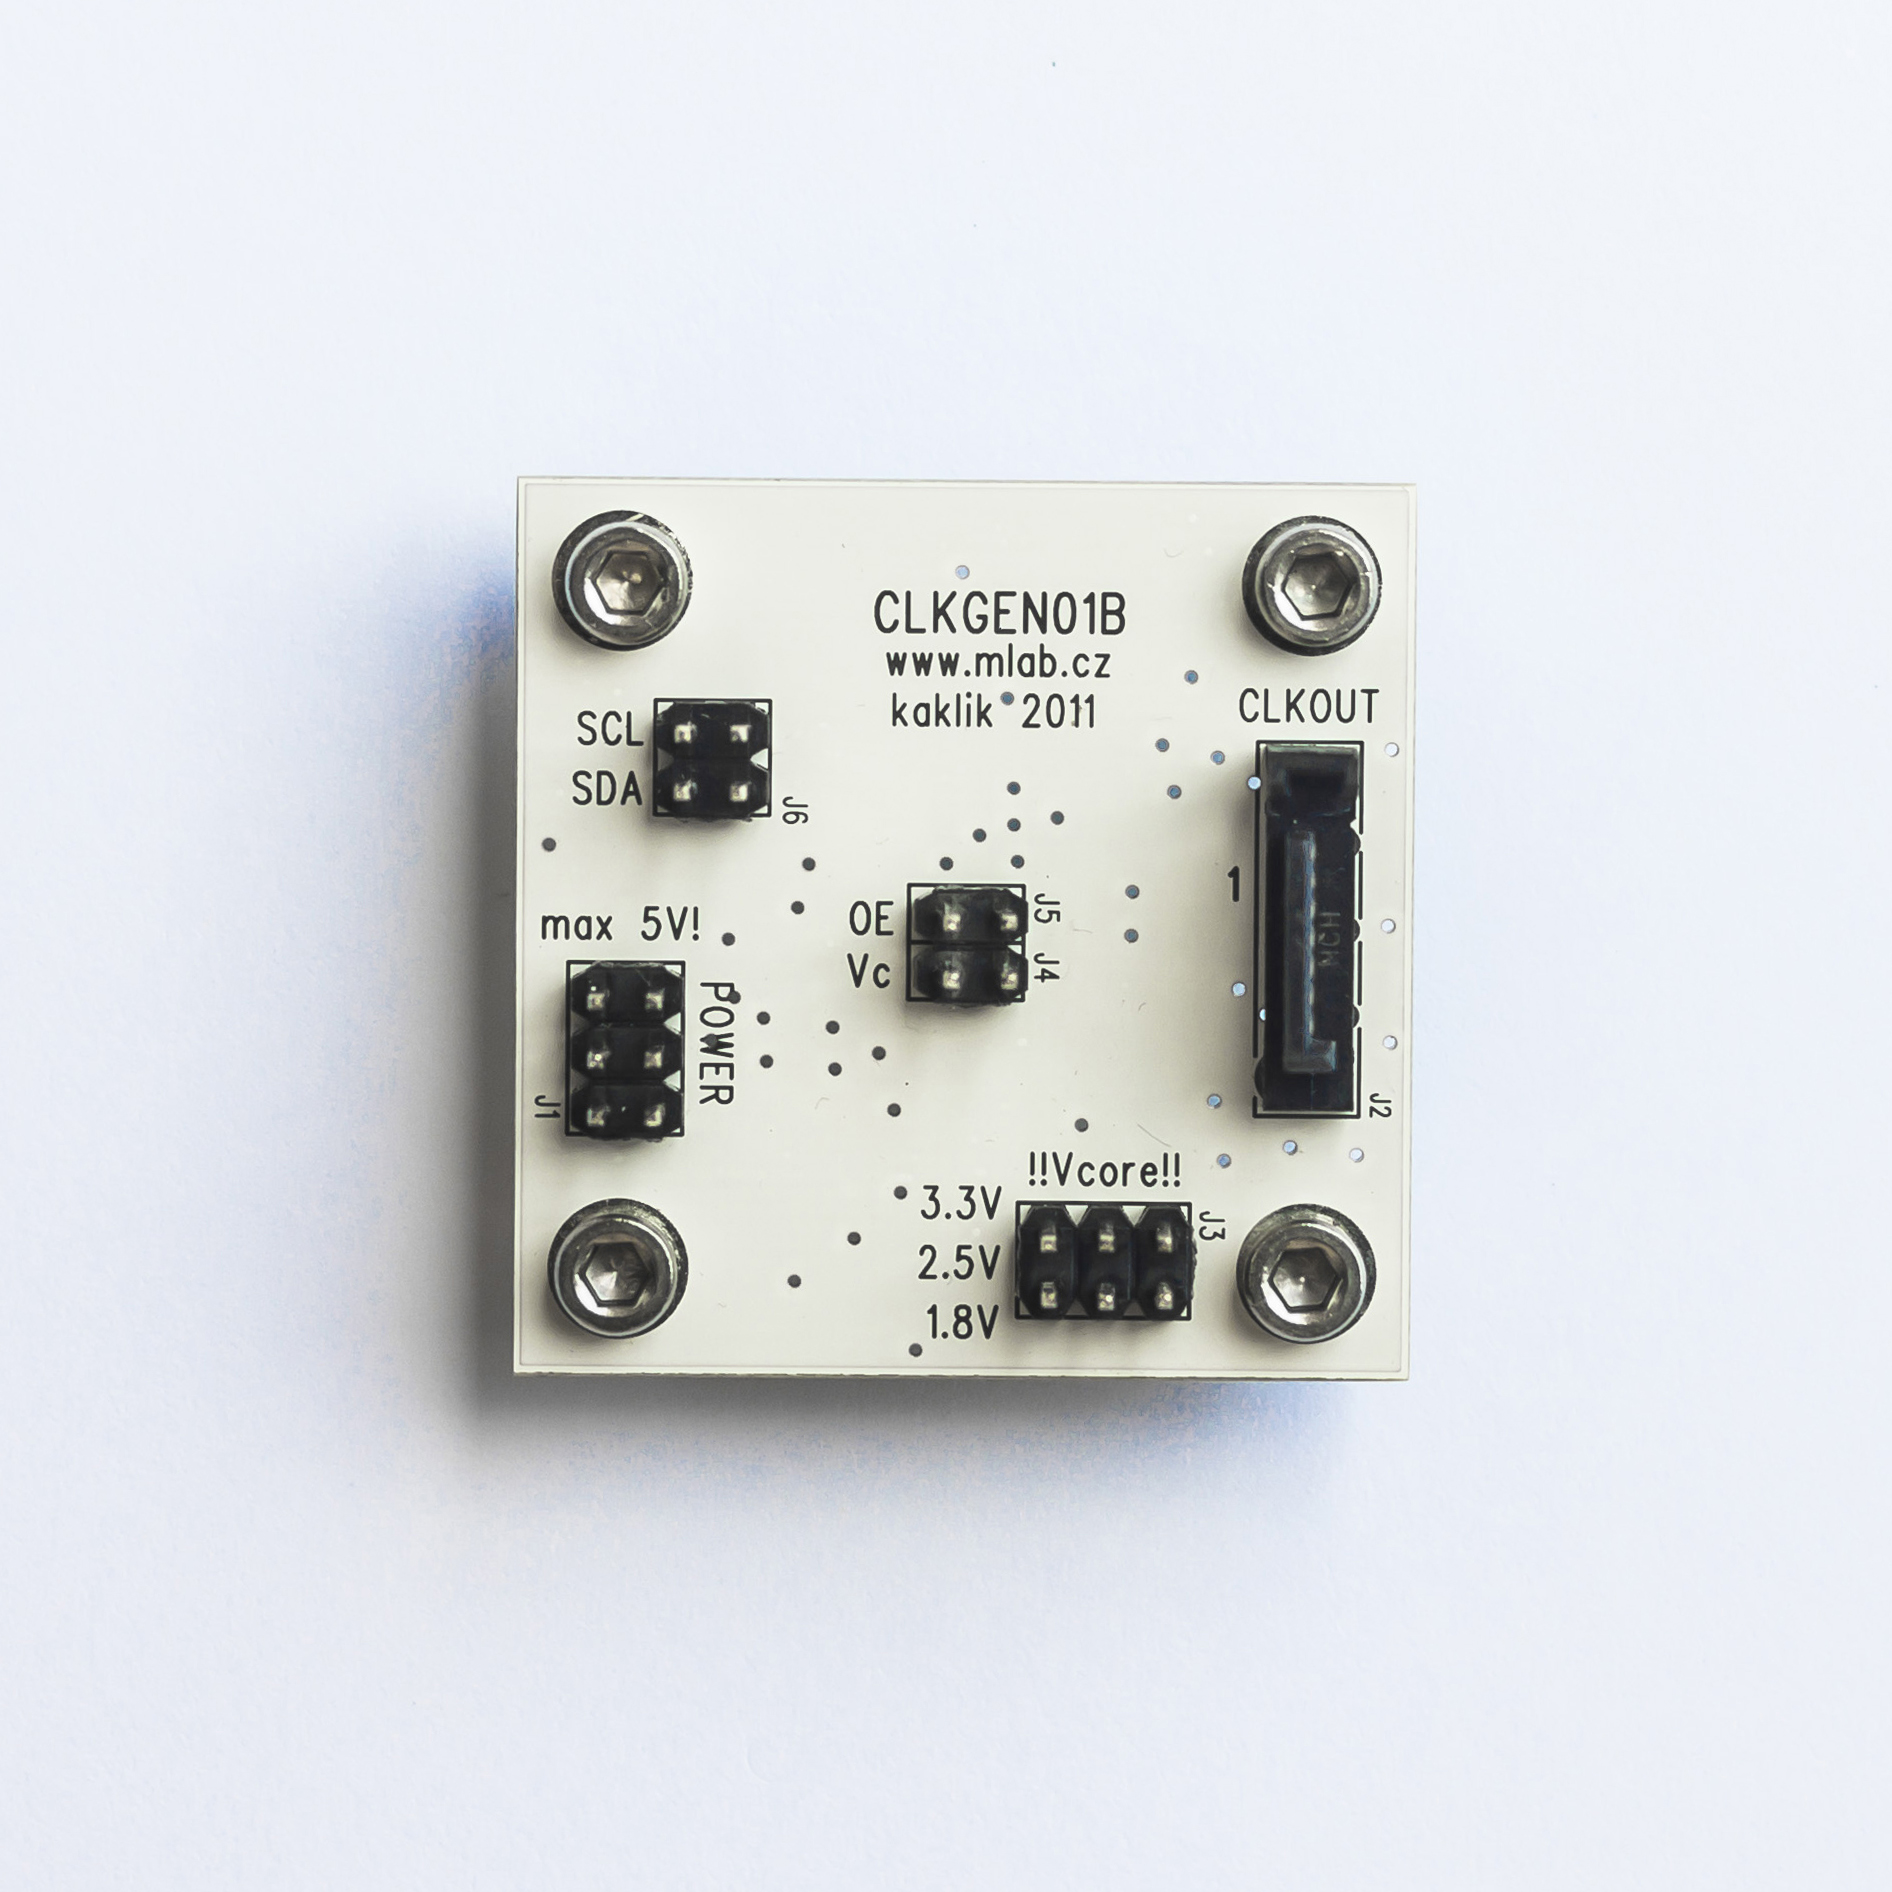
\includegraphics [width=80mm] {./img/CLKGEN01B_Top_Big.jpg} 
\end{center}
\end{figure}

\tableofcontents

\section{Technické parametry}
\begin{table}[htbp]
\begin{center}
\begin{tabular}{|c|c|p{4.7cm}|}
\hline
Parametr & Hodnota & Poznámka \\
\hline
Napájecí napětí POWER  & max 5V &  160mA \\ 
\hline
Napájecí napětí Vcore & +1,8V, 2,7V, 3,3V &  Záleží na konkrétním typu čipu Si5XX \\ 
\hline
Frekvenční rozsah  & 10 - 1500 MHz & Záleží na konkrétním typu čipu Si5XX, obvykle 10-810MHz \\ 
\hline
Fázový jitter  & $<$ 0,3ps & Pro obvody řady Si570 \\ 
\hline
\end{tabular}
\end{center}
\end{table}

\section{Popis konstrukce}

\subsection{Zapojení}
Zapojení modulu je řešeno tak, aby umožnilo připojení řídícího mikroprocesoru provozovaného na stejném i jiném napájecím napětí vůči čipu Si5XX. V konstrukci je proto využit převodník napěťových úrovní, který může být při jeho absenci přemostěn dvěma nulovými odpory R4 a R5.

V případě provozování modulu na napájecím napětí různém od napájecího napětí Si570 si modul může stabilizovat napájení sám díky lineárnímu stabilizátoru. V takovém případě je ale přesto dát pozor, aby napájení nepřesáhlo dovolené napětí na translátoru, tedy hranici 5V. 

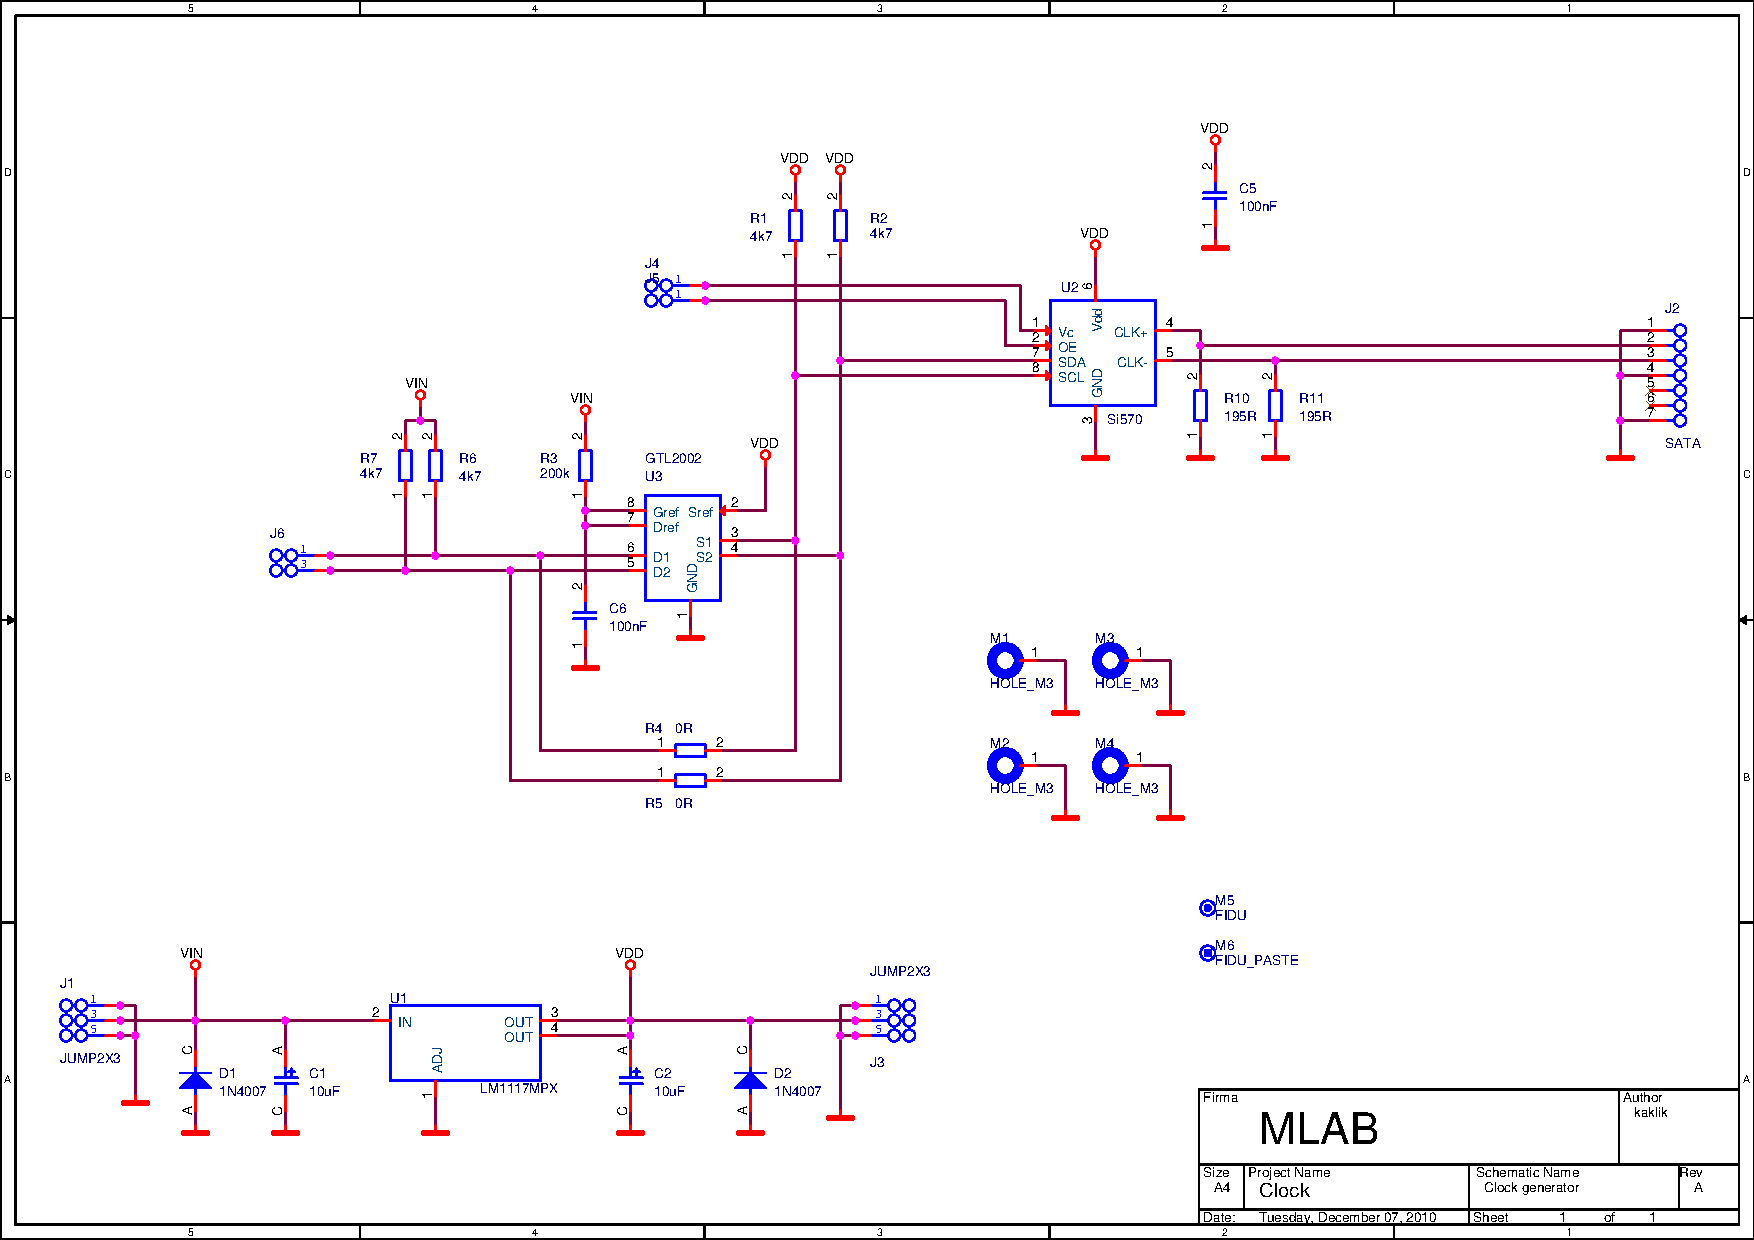
\includepdf[pages={1},landscape=true]{../../SCH/CLKGEN.pdf}

Jak je vidět ze zapojení, výstup je předpokládán diferenciální, avšak není problém osadit verzi čipu Si570 s CMOS výstupem. 

\subsection{Odrušení}

Vzhledem k tomu, že modul je ze své podstaty generátorem signálu, je s ním i třeba tak pracovat a dbát na dostatečné odrušení vůči jiným součástem aparatury. Tomuto výrazně pomáhá vhodná volba základní desky, z MLABu nejlépe ALBASE.

\subsection{Mechanická konstrukce}

Modul klasicky předpokládá uchycení na čtyřech šroubech, z důvodu vhodného odstínění je vhodné zabezpečit aby všechny šrouby byly vodivě spojeny s podložkou.  

\section{Výroba a testování}
Modul je z z důvodu zabezpečení kvalitního blokování i na vysokých frekvencích (až 1,5GHz) navržen na dvouvrstvém silně prokoveném plošném spoji. A proto je obtížná jeho amatérská výroba.

\subsubsection{Osazení}

Modul je možné osadit i ručně, avšak je třeba dbát zvýšené opatrnosti kvůli elektrostatickým nábojům, neboť čipy Si570 je snadné poškodit.

\begin{figure} [htbp]
\begin{center}
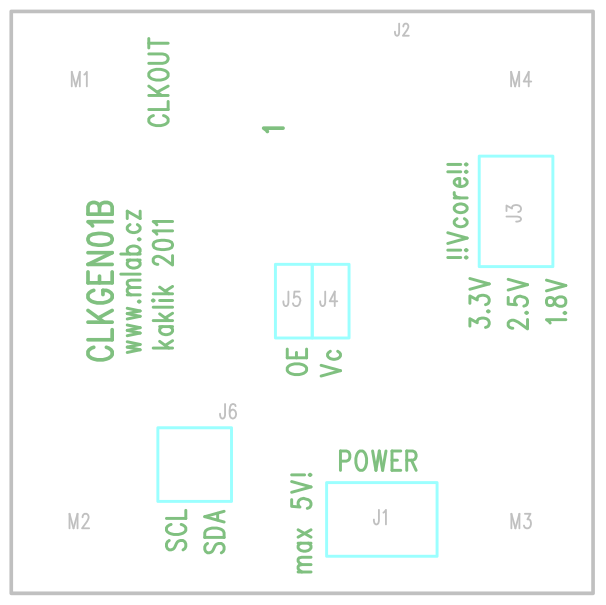
\includegraphics [width=75mm] {./img/O1.png} 
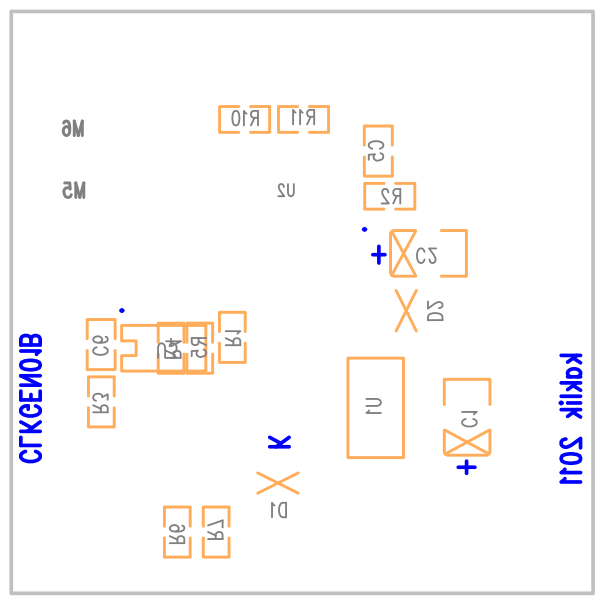
\includegraphics [width=75mm] {./img/O2.png} 
\end{center}
\end{figure}

Odpory R2 a R4 se osazují jen v případě že se neosazuje U3.

\begin{center}
\begin{tabular}{|c|c|c|c|}
\hline 
Počet & Označení & Typ  & Pouzdro  \\ 
\hline 
2 & C1,C2 & 10uF & Elyt-B \\
2 &	C5,C6 & 100nF & 0805 \\
2 &	D1,D2 & 1N4007 & SMA \\
2 & J1,J3 & JUMP2X3 & Pinheader \\
1 &	J2 & SATA-connector & \\ 
2 &	J4,J5 & JUMP2X1 & \\
1 &	J6 & JUMP2X2 & \\
4 & R1,R2,R6,R7 & 4k7 & 0805 \\
1 &	R3 & 200k & 0805 \\
2 &	R4,R5 & - 0R & 0805\\
2 &	R10,R11 & 195R & 0805 \\
1 &	U1 & LM1117MPX & SOT-23 \\
1 & U2 & Si570 & 5x7 mm \\
1 &	U3 & GTL2002 & SO8 \\
\hline 
\end{tabular} 
\end{center}


\subsubsection{Nastavení}
Při připojení modulu k napájení generuje frekvenci nastavenou při výrobě v Silicon Labs. Je ale možné zpřesnit generovanou frekvenci. K tomu je nutné zprovoznit komunikaci přes I2C sběrnici. 

\section{Programové vybavení}
V kombinaci s jinými moduly, lze generátor ladit z počítače. Jedním z nejjednodušších řešení je použít modul PIC18F4550v01A a firmware ze zdroje \cite{DG8SAQemulator} pak lze k ladění použít jakýkoli software pracující s konstrukcí \cite{DG8SAQSynthesizer}, například USBSynth \cite{USB_Synth}.


\begin{thebibliography}{99}
\bibitem{Si570board}{Původní konstrukce Si570 Board } 
\href{http://wb6dhw.com/inactive.html}{http://wb6dhw.com/inactive.html}

\bibitem{DG8SAQemulator}{PIC emulátor USB syntezátoru od DG8SAQ} 
\href{http://www.qrpradio.org/pub/softrocks/manuals/Softrock Group Files 210109/21 9V1AL/02 UBW Emulator/README.txt}{http://www.qrpradio.org/pub/softrocks/manuals/Softrock Group Files 210109/21 9V1AL/02 UBW Emulator/README.txt}

\bibitem{DG8SAQSynthesizer}{Wideband RF Synthesizer} 
\href{http://www.mydarc.de/dg8saq/SI570/index.shtml}{http://www.mydarc.de/dg8saq/SI570/index.shtml}

\bibitem{USB_Synth}{USB Synth}
\href{ http://www.mydarc.de/dg8saq/hidden/USB\_Synth3.zip}{http://www.mydarc.de/dg8saq/hidden/USB\_Synth3.zip}

\end{thebibliography}
\end{document}